\chapter{Ausgangssituation}
\label{chap:three}
Im folgenden Kapitel wird die wissenschaftliche Spezialbibliothek des \textit{Max-Planck-Institutes für empirische Ästhetik} porträtiert, um die Ausgangslage zu umreißen.
Anschließend werden die bibliothekarischen Informationsdienstleistungen der Bibliothek skizziert und der Frage nachgegangen, 
welche statistischen Daten aggregiert und ausgewertet wurden. Diese Daten stellen die Basis für die spätere Konzeption und Entwicklung eines datengetriebenen Unterstützungssystems dar.

\section{Bibliothek}
\label{chap:three_one}
\subsection{Allgemeines}
%Wann wurde die Bibliothek gegründet?\\
Die Spezialbibliothek wurde im Zuge der Gründung des \textit{\acrshort{MPI EA}}
in Frankfurt im Jahr 2013 gegründet. Die Aufgabe des Institutes ist die interdisziplinäre Erforschung 
empirischer Fragestellungen der Ästhetik. Das Institut besteht derzeit aus drei Abteilungen \textit{Sprache und Literatur}, 
\textit{Musik} und \textit{Neurowissenschaften} sowie einigen Forschungsgruppen. %Ungefähr 150 Mitarbeiter:innen 
%arbeiten in dem Institut. 



% Warum wurde die Bibliothek gegründet?
%Welche Aufgaben hat die Bibliothek?
%Welche Servicedienstleistungen bietet die Bibliothek an?
Die Bibliothek ist eine Serviceeinrichtung des Institutes und dient mit ihren Informationsdienstleistungen 
der Forschung.
Zentral ist dabei die Informationsversorgung der Forschenden. Die benötigten Informationen sind Bücher, 
Zeitschriften, Zeitschriftenartikel sowohl in gedruckter als auch in elektronischer Form.
%Seit der Institutsgründung wird neben des nutzungsorientierten Bestandaufbaus ebenfalls eine planmäßige 
%Bestandsentwicklung betrieben. Das Erwerbungsprofil der Bibliothek leitet sich aus dem Forschungsauftrag des Institutes 
%ab und umfasst dementsprechend die Erwerbung von Informationsressourcen, die sich den theoretischen und 
%empirischen Fragestellungen der Ästhetik widmen.
%Wie groß ist der Bibliotheksbestand? 
Der Bibliotheksbestand ist somit hybrid. Er besteht sowohl aus gedruckten als auch Online-Medien sowie 
audiovisuellen Materialien. An Bestand umfasst die Bibliothek zirka 11.000 Bücher, 30 laufende Zeitschriften, 
knapp über 200 audiovisuelle Medien sowie Online-Datenbanken
und Online-Zeitschriften.

\subsection{Organisatorische Einbettung}
%Wie sieht der größere Organisationsrahmen der Bibliothek aus?\\
Um alle Informationsbedarfe der Forscher:innen zu befriedigen, wird die Bibliothek in ihren Aufgaben von der
\textit{\acrlong{mpdl}} unterstützt. Deren Portfolio umfasst vorrangig die zentrale 
Lizenzierung von relevanten elektronischen Informationsressourcen, die Bereitstellung von Softwarelösungen, 
das Betreiben des Publikationsrepositoriums \textit{\acrshort{PuRe.MPG}} der \textit{\acrfull{MPG}} sowie
das Vorantreiben von Open-Access-Initiativen. 

Darüber hinaus ist die Spezialbibliothek Teil des \textit{\acrshort{HeBis}-Verbundes}. 
Seit Ende 2014 finden die Geschäftsprozesse der Katalogisierung und der Erwerbung im \textit{\acrfull{CBS}} und 
im Lokalsystem \textit{\acrfull{LBS}} vom \textit{\acrshort{OCLC}} statt. Im \textit{\acrfull{OPAC}} befinden sich Bücher, ausgewählte E-Books 
und Zeitschriften (Print und Online) der Institutsbibliothek. Lokal lizenzierte Datenbanken finden sich dagegen
nicht im Katalog. Das \textit{\acrshort{LBS}} wird gehostet und betreut 
vom Lokalsystem-Team Frankfurt. Als Service-Leistungen werden der Bibliothek besondere Funktionalitäten 
für das \textit{\acrlong{CBS}} und Statistiken aus dem \textit{\acrshort{LBS}} von dem Lokalsystem-Team bereitgestellt.


\subsection{Informationsdienstleistungen}
Das Bibliotheks-Team des \textit{\acrshort{MPI EA}} ist verantwortlich für den Ablauf und Organisation der bibliothekarischen 
Informationsdienstleistungen. Eine Übersicht der Informationsdienstleistungen,
aufgeschlüsselt nach den Basisfunktionen einer Bibliothek \cite[S. 204 f.]{rosch_bibliotheken_2019}, zeigt \autoref{tab:Informationsdienstleistungen}. 
Die zentralen Informationsdienstleistungen der Spezialbibliothek bestehen aus der Sammeltätigkeit und dem Benutzungsservice.
Seit der Institutsgründung wird neben dem nutzungsorientiertem Bestandaufbau ebenfalls eine planmäßige 
Bestandsentwicklung betrieben. Das Erwerbungsprofil der Bibliothek leitet sich aus dem Forschungsauftrag des Institutes 
ab und umfasst dementsprechend die Erwerbung von Informationsressourcen, die sich den theoretischen und 
empirischen Fragestellungen der Ästhetik widmen.


Die Dienstleistungsbereiche der Benutzung sind zuständig für die Organisation der Fern- und Ortsleihe 
von Informationsressourcen, die nicht in das Erwerbungsprofil der Spezialbibliothek fallen. Ferner sind diese 
für die Informationsbeschaffung sowohl über Dokumentenlieferdienste als auch für die Akquise von einzelnen Zeitschriftenaufsätzen zuständig.

\begingroup
\setlength{\tabcolsep}{12pt} % Default value: 6pt
\renewcommand{\arraystretch}{1.5} 
\begin{table}[h]
    \centering
    \begin{adjustbox}{max width=\textwidth}
    \begin{tabular}{p{0.4\textwidth}p{0.9\textwidth}}
       \toprule
       \textbf{Basisfunktion}          & \textbf{Beschreibung}\\
       \midrule
        Benutzung                               &Ausleihe, Lesesaalnutzung, Organisation der Lieferdienste (Fern und Ortsleihe, Dokumentenlieferdienste)\\
        Management techn. Infrastruktur         &\textit{\acrshort{PuRe.MPG}}, Medien-Datenbank\\
        Ordnen                                  &Aufstellungssystematik (RVK)\\
        %Sammeln bes. Materialien                &Stimulus wie Musikstücke, Bilder, Textlizenzen, Zeitschriftenartikel\\
        Sammeln und Erschließen                 &geplanter Bestandsaufbau, Integrierter Geschäftsgang Medienerwerbung und Medienerschließung, besondere Materialien\\
        Vermitteln                              &Literaturrecherche, Nutzung elektronischer Ressourcen, Urheberrecht und Publikationsberatung\\
   
       \bottomrule
    \end{tabular}
    \end{adjustbox}
    \caption
    \end{table}
\endgroup

Weitere Informationsdienstleistungen sind die Betreuung des Publikationsrepositoriums \textit{\acrshort{PuRe.MPG}} des Institutes, spezielle Beratungsdienstleistungen 
zum Urheberrecht und zum Publishing sowie klassische Auskunfts- und Informationsdienste. Seit Beginn 2016 
geschieht die Ausleihe der Medien über ein Selbstverbuchungssystem.\\
%Nutzergruppen

\subsection{Evaluation der Informationsdienstleistungen}

Zu fast jeder Informationsdienstleistung der Spezialbibliothek werden quantitative Daten elektronisch generiert. 
\autoref{tab:Statistische_Daten} zeigt Daten, die bereits jetzt in der ein oder anderen Form aggregiert und ausgewertet werden. 
Die Tabelle stellt nach den Evaluationstypen dar, ab wann und wie regelmäßig die Statistiken erfasst werden. Ferner bietet sie einen Überblick darüber, in welchem 
Format die Daten vorliegen, über die Quellen aus der die Daten stammen und ob die Daten bereits systematisch ausgewertet und/oder visualisiert werden.


\begingroup
\setlength{\tabcolsep}{4pt} % Default value: 6pt
\renewcommand{\arraystretch}{1.5}
%\resizebox{\textwidth}{!}{
\begin{table}[h]
    \centering
    \begin{adjustbox}{max width=\textwidth}
    \Huge
    \begin{tabular}{lllclllcc}
      %\begin{tabular}{p{3cm}p{5cm}p{1cm}p{1.5cm}p{2cm}p{4cm}}
       \toprule
       \textbf{Evaluationstyp} &\textbf{Basisfunktion}               &\textbf{Daten}                                 &\textbf{Zeitraum} &\textbf{Turnus}    &\textbf{Quelle}  &\textbf{Format}          &\textbf{Syst. Auswertung} & \textbf{Visualisierungen}\\
       \midrule     
            Nutzungsbezogen         &Benutzung                      & Ausleihzahlen Bibliotheksbestand              & 2016-             & monatlich         & LBS          & Mail, xlsx                & nein  & -\\
            Nutzungsbezogen         &Benutzung                      & Ausleihzahlen Lieferdienste                   & 2015-             & monatlich         & intern       & xlsx                      & ja    & teilweise, Liniendiagramm\\ 
            Nutzungsbezogen         &Benutzung                      & Besonders nachgefragte Medien (OPAC)          & 2017-             & monatlich         & LBS          & Mail, txt                 & nein  & -\\ 
            Nutzungsbezogen         &Sammeln                       &\acrshort{COP 5}-Statistiken elektr. Ressourcen& 2013-            & unbekannt                 & mpdl         & csv, tsv, txt             & nein  & -\\ 
            Nutzungsbezogen         &Benutzung                      & Lesesaalnutzung                               & 2015-             & wöchentlich       & intern       & xlsx                      & nein  & -\\ 
            %Sammeln bes. Materialien        & Anzahl der Materialien                       & unregelmäßig      & unregelmäßig      & intern       & xlsx                      & nein  & -\\
            Sammlungsbezogen         &Sammeln                       & Budget nach Kostenstellen                   & 2018-               & monatlich         & LBS          & Mail, txt                 & ja    & -\\ 
            Sammlungsbezogen         &Sammeln                       & Umsatz nach Lieferanten                     & 2018-               & monatlich         & LBS          & Mail, txt                 & ja    & Balken- und Kreisddiagramm\\ 
            Sammlungsbezogen         &Sammeln                       & Größe und Art des Bestandes                   & 2014-             & jährlich          & LBS, intern  & csv                       & nein  & -\\ 
            Sammlungsbezogen         &Sammeln                       & Neuerwerbungslisten                           & 2014-             & monatlich         & LBS, intern  & tsv                       & nein  & -\\ 
            

        \bottomrule
    \end{tabular}
    \end{adjustbox}
    \caption
    \label{tab:Statistische_Daten}
    }
     \end{table}
\endgroup


Intern erfasst die Bibliothek monatlich die Daten der Ausleihe über die Lieferdienste. Unterschieden 
wird in der Erfassung nach Medientypen, nach Ausleihort und Ausleihart. Zudem werden wöchentlich 
Statistiken zur Nutzungshäufigkeit des Lesesaals geführt. Jährlich wird die Bestandsgröße nach 
Medientyp für die Buchhaltung ermittelt.

Die Ausleihzahlen des Bibliotheksbestandes werden bei Bedarf durch das Lokalsystem-Team ermittelt und an die Bibliothek geschickt. 
Diese liegen kumulativ nach Ausleihanzahl des einzelnen Titels oder nach Jahr und der Identifikationsnummer des Titeldatensatzes im 
\textit{\acrshort{CBS}} vor. Ebenfalls stehen die Ausleihzahlen als Rohdaten, in denen jede Titelausleihe aufgeführt wird, zur Verfügung.
%Ausgewertet wurden die Ausleihzahlen bisher noch nicht.

\begin{figure}[H]
    \centering
        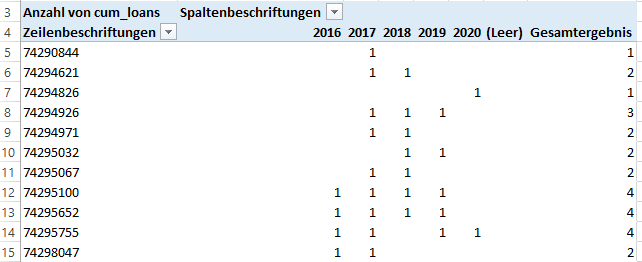
\includegraphics[width=8cm, height=4.0cm]{ausleihzahlen_epn_jahr}
        %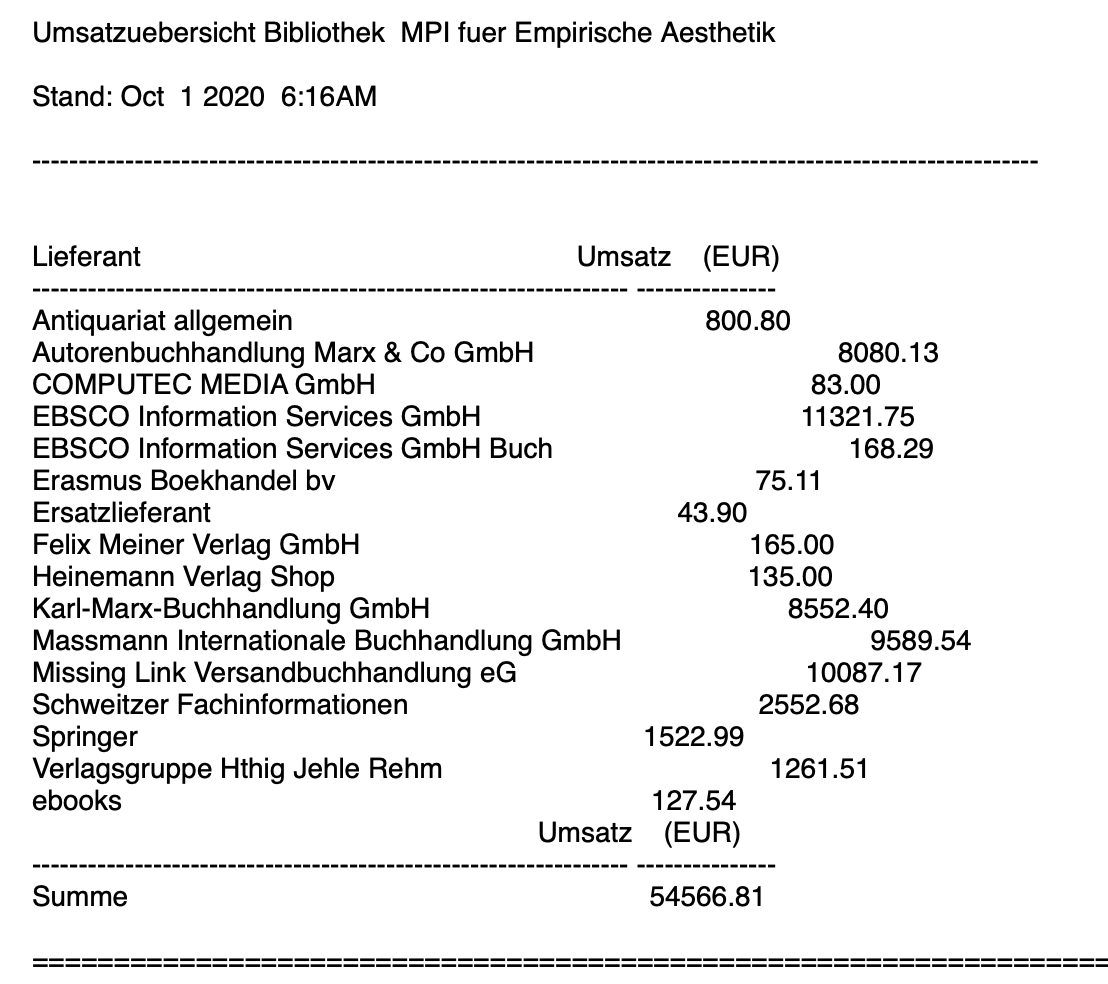
\includegraphics[width=6.5cm, height=6cm]{umsatzuebersicht}
        \caption{Anzahl der Titelausleihen nach Identifikationsnummer und Jahr}
        \label{fig:Titelausleihen}
\end{figure}


Monatlich bekommt die Bibliothek kumulative Budget- und Umsatzübersichten der Kostenstellen und der Lieferanten zugeschickt. 
Die Kostenstellen bilden die einzelnen Abteilungen und zum Teil die Forschungsgruppen des Institutes ab. 
Bearbeitet werden nur die Umsatzübersichten der Lieferanten, um die Umsatzverteilung nach Lieferanten zu steuern.
\autoref{fig:budget- und umsatzuebersicht} zeigt die Budget- und Umsatzübersichten, die vom Lokalsystem-Team als email zur Verfügung gestellt werden.


\begin{figure}[h]
    \centering
        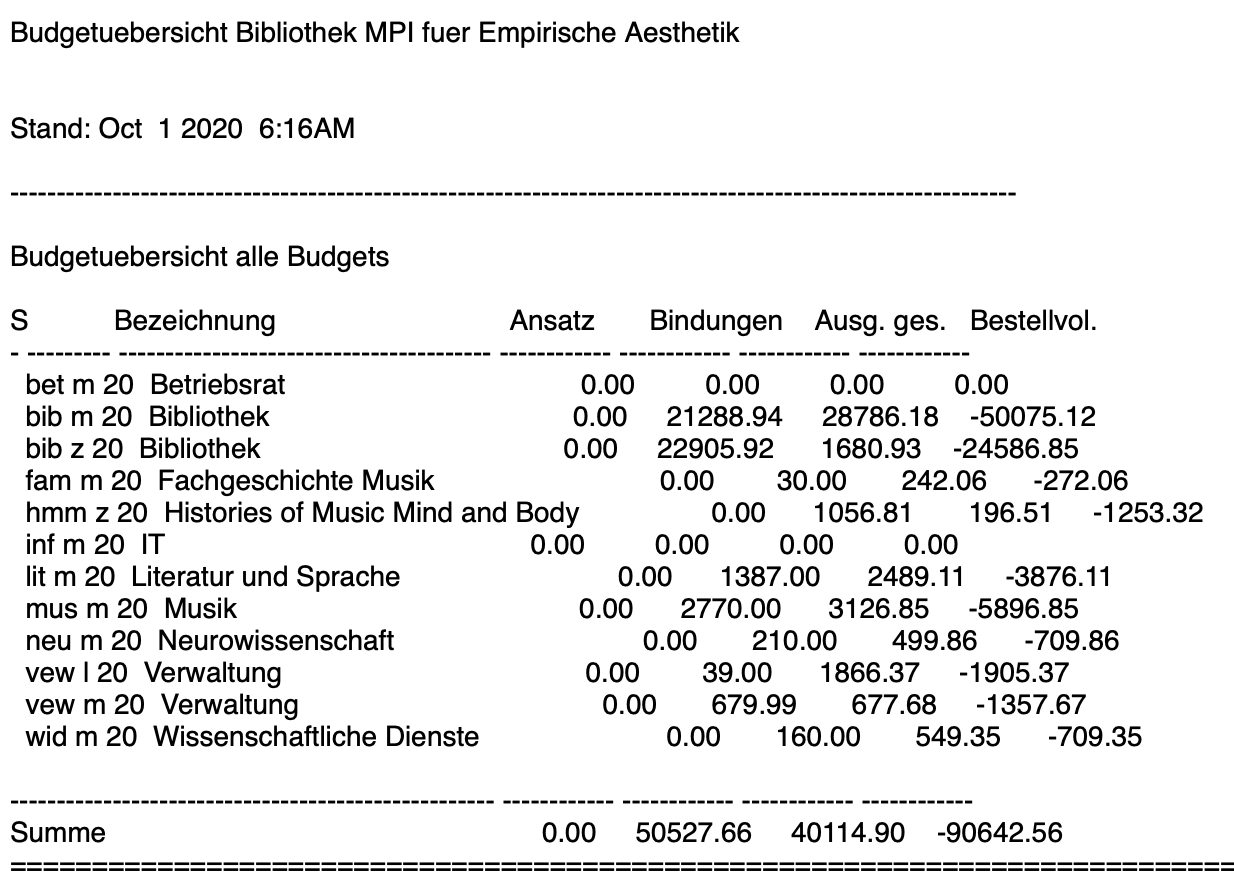
\includegraphics[width=6.5cm, height=7.0cm]{budgetuebersicht}
        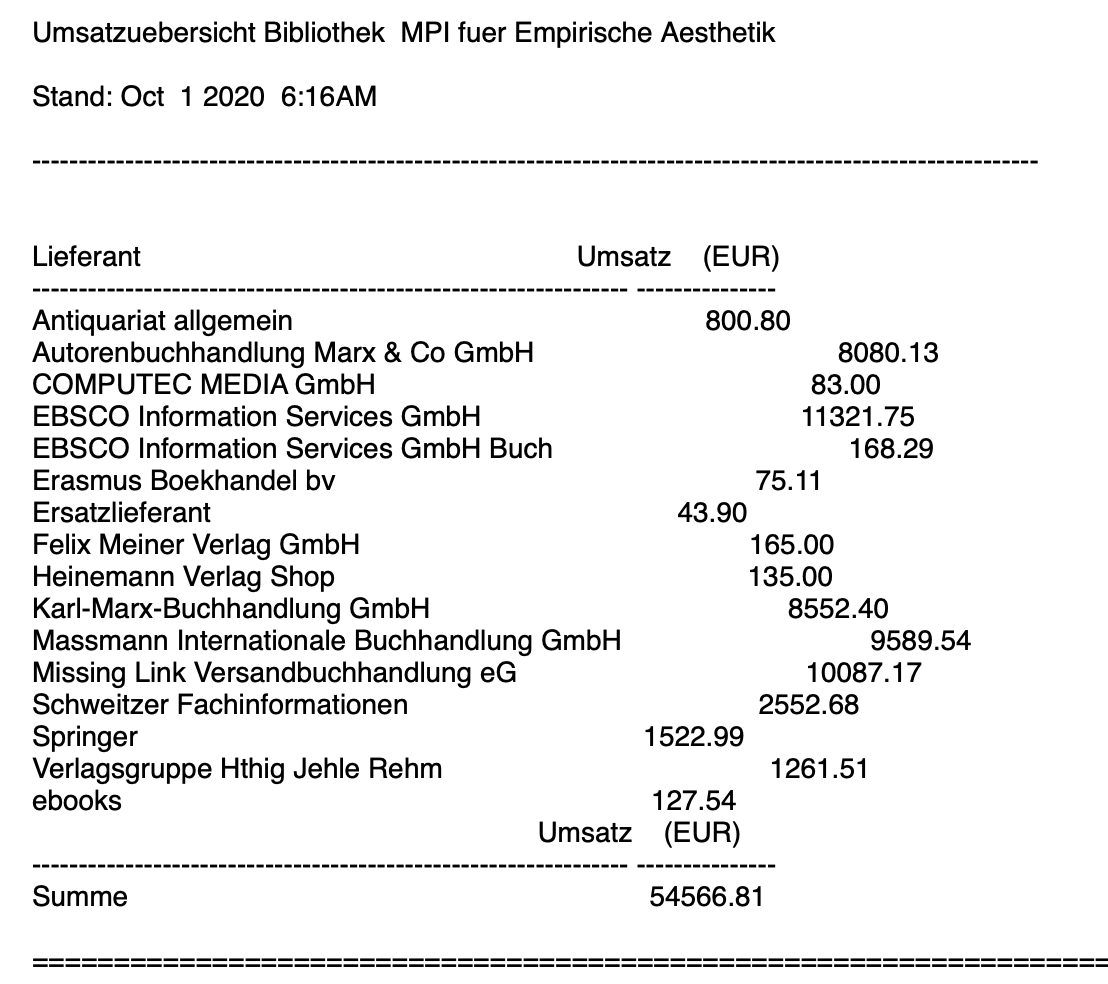
\includegraphics[width=6.5cm, height=7.0cm]{umsatzuebersicht}
        \caption{Monatliche Budget- und Umsatzübersicht}
        \label{fig:budget- und umsatzuebersicht}
\end{figure}

Die Ausgaben für die lokal lizenzierten Datenbanken fehlen in der Aufstellung der Ausgaben und werden in einer Tabelle extra geführt.

Die \textit{\acrfull{COP 5}} der Verlage werden auf einen internen Portal von der \textit{\acrshort{mpdl}} dem Institut zur Verfügung gestellt.
Diese Statistiken verzeichnen den Zugriff innerhalb der IP-Adressbereiche des Institutes auf die elektronische Ressourcen, 
die konsortial durch die \acrshort{MPG} lizenziert wurden. Darunter fallen ebooks der Verlage 
\textit{Springer}, \textit{Wiley} oder \textit{De Gruyter}. Bisher wurden diese von der Bibliothek noch nicht gesichtet und ausgewertet.
% Von seitens der Bibliothek wurden diese Statistiken leider noch nicht angefasst.

Eine proaktive und systematische Auswertung der Entwicklung der Bestandsgröße, der Ausleihzahlen und der \textit{\acrshort{COP 5}}-Statistiken findet nicht
oder nur unzureichend statt. Auch wird das Potential wie in \autoref{chap:two_one} beschrieben hinsichtlich der Budgetplanung
nicht ausgeschöpft.

%\section{Zusammenfassung}

